\documentclass[a4 122pt]{article}

\usepackage{color}
\usepackage{polski}
\usepackage[utf8]{inputenc}
\usepackage{amsmath}
\usepackage{amsthm}
\usepackage{todonotes}
\usepackage{geometry}
\usepackage{hyperref}

\usepackage{floatrow}

\geometry{
  body={6.5in, 8.5in},
  left=0.7in,
  top=0.8in,
  bottom=0.8in
}
%\usepackage[pdftex]{graphicx}
\usepackage{sidecap}
\usepackage[linesnumbered, vlined]{algorithm2e}


\usepackage{tikz}
\usepackage{tikz,fullpage}
\usetikzlibrary{arrows,%
                petri,%
                topaths}%
\usepackage{tkz-berge}
\usepackage[position=top]{subfig}

\newtheorem{twierdzenie}{Twierdzenie}
\newtheorem{definicja}{Definicja}
% zmiana caption dla algorytmu
\usepackage{caption}% http://ctan.org/pkg/caption
\newenvironment{algorytm}[1][htb]
  {\renewcommand{\algorithmcfname}{Algorytm}%
   \begin{algorithm}[#1]%
  }{\end{algorithm}}


\title{Planarność grafu}
\author{Paweł Sokołowski\\Michał Kaszlej}



\begin{document}




\maketitle

	\section{Cel projektu}

		Celem projektu jest napisanie algorytmu heurystycznego sprawdzającego czy zadany graf jest planarny.
		Według twierdzenia Wagnera podanego w książce W.R Wilsona "Wprowadzenie do teorii grafów"[1]:

		\begin{figure}[h]
			\begin{center}
				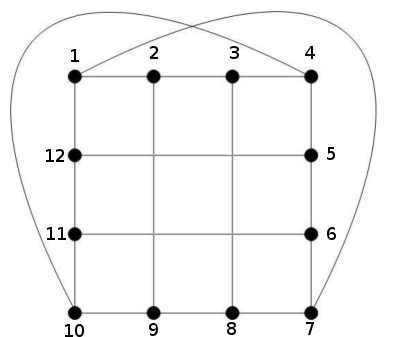
\includegraphics[width=0.5\textwidth]{include/graf.png}
				\caption{Zadany graf}
			\end{center}
		\end{figure}



\floatsetup[figure]{capposition=beside,capbesideposition={top,right}}

		\begin{twierdzenie}
		Dany graf jest planarny wtedy i tylko wtedy, gdy nie zawiera podgrafu ściągalnego do grafu $K_{3.3}$ lub do grafu $ K_5 $
		\end{twierdzenie}

	\section{Język programowania} 

		Algorytm zostanie zaimplementowany za pomocą języka C\#.

	\section{Algorytm}

		Algorytm rozwiązujący zadany problem zostanie wybrany w dalszej fazie projektu.

	\pagebreak

	\section{Opis algorytmu}	
	Algorytmem, który zostanie zaimplementowany w celu sprawdzenia czy zadany graf jest planarny jest test planarności przy użyciu twierdzenia Wagnera[1, r 85]:
	\begin{twierdzenie}
	Dany graf jest planarny wtedy i tylko wtedy, gdy nie zawiera podgrafu ściągalnego do grafu $K_{3.3}$ lub do grafu $ K_5 $
	\end{twierdzenie}
	Implementacja algorytmu wywodzi się wprost z powyższego twierdzenia. 
	Polegała będzie ona na dokonywaniu operacji ściągania grafu do podgrafu o 5 lub 6 wierzchołkach.
	Jeżeli uda się w ten sposób utworzyć graf $ K_5 $ lub $K_{3.3}$ oznaczało to będzie, że wejściowy graf nie jest planarny.
	Poniżej znajduje się pseudokod algorytmu.
	
	\begin{algorytm}[H]
	\newcommand{\forcond}{$i=0$ \KwTo $n$}
	\SetKwFunction{Fn}{JestPlanarny}
	\Fn{graf g}\Begin{
	
		\KwData{Testowany graf}
		\KwResult{Czy testowany graf jest planarny}
		\If{g posiada 6 wierzchołków}{
			Sprawdź czy graf jest $K_{3.3}$\;
		}
		\If{g posiada 5 wierzchołków}{
			Sprawdź czy jest $K_5$\;
		}
		\If{graf posiada więcej niż 5 wierzchołków}{
			\ForEach{krawędź e grafu g}{
				h $\leftarrow$ zbuduj graf poprzez ściągnięcie krawędzi e z grafu g\;
				\Fn{h}\;
			}
		}
	}
	\caption{Pseudokod algorytmu}
	\end{algorytm}
	
	Linie 1-6 algorytmu wydają się dosyć oczywiste. 
	Jeżeli mamy do czynienia z grafem pięcio lub sześcio wierzchołkowym sprawdzane jest odpowiednio czy nie jest to odpowiednio $K_5$ lub $K_{3.3}$. 
	W linii 8 następuje iteracja po wszystkich krawędziach grafu. 
	Najistotniejszym fragmentem algorytmu wydaje się być linia 9. 
	Budowany jest tam nowy graf poprzez "ściągnięcie" danej krawędzi. 
	Sama operacja zostanie opisana w dalszej części pracy.
	
	\subsection{Operacja ściągnięcia}
		Ściąganie wzdłuż krawędzi polega na utożsamianiu wierzchołków, które łączy dana krawędź i pomijaniu ewentualnych pętli. 
 		
		\begin{definicja}
			Mówimy, że graf $G_1$ jest ściągalny do $G_2$, jeśli $G_2$ można otrzymać z $G_1$ poprzez skończony ciąg operacji ściągania wzdłuż krawędzi.
		\end{definicja}
		
		Z \textbf{Twierdzenia 1} wiemy, że jeżeli uda nam się ściągnąć graf wejściowy do $K_5$ lub $K_{3,3}$ to nie jest planarny. 
	
	\subsection{Struktury danych}

		Graf reprezentowany będzie za pomocą listy sąsiedztwa. 
		W reprezentacji tej, struktura przedstawiająca wierzchołek będzie składała się z jego identyfikatora oraz listy jego sąsiadów. 
		Sam graf będzie zbudowany z listy wierzchołków. 
		Reprezentacja ta pozwoli na budowanie grafu poprzez ściągnięcie krawędzi w czasie $O(m)$.
	
	\subsection{Historia operacji}
		Celem zadania jest próba znalezienia podgrafu ściągalnego do $K_5$ lub $K_{3,3}$, aby odpowiedzieć na pytanie czy dany graf jest planarny. 
		Nie wystarczy więc aby projektowany algorytm zwracał jedynie binarną odpowiedź, tak lub nie, musi w przypadku stwierdzenia nieplanarności zwrócić podgraf ściągalny do $K_5$ lub $K_{3,3}$.
		Aby mieć możliwość odtworzenia takiego podgrafu (w trakcie działania algorytmu zmieniana jest struktura grafu, usuwane są krawędzie i wierzchołki) podczas każdego zejścia rekurencyjnego zapamiętywana będzie historia ściągniętych krawędzi. 
		Umożliwi to odtworzenie szukanego podgrafu w zadanym grafie.
	
	\subsection{Złożoność}
	
		Istnieje, szereg algorytmów pozwalających na sprawdzenie planarności grafu.
		Od roku 1974 istnieją algorytmy o złożoności liniowej $O(n)$ w tym np. metody Hopcroft, Tarjan[2] czy Boye, Myrvold[3].
		Są to metody bardzo skomplikowane, wymagające żmudnej, czasochłonnej implementacji.
		
		Prostszy w implementacji jest algorytm korzystający z obserwacji dotyczących cyklów i segmentów w grafach planarnych. 
		Jest on mniej wydajny niż wspominane powyżej algorytmy, ale jego złożoność jest również wielomianowa - rzędu $O(n^3)$. 
		Niestety, algorytm ten nie mógł być zastosowany, ponieważ w przypadku stwierdzenia nieplanarności nie zwraca on podgrafu ściągalnego do $K_5$ lub $K_{3, 3}$.
		
		Jako, że zadanie projektowe zdefiniowane zostało dla grafu o 12 wierzchołkach - zdecydowaliśmy, że zastosowanie tak skomplikowanych algorytmów nie jest tu zasadne. 
		Zaprezentowane w niniejszej pracy rozwiązanie osiąga wydajność na poziomie $O(m!)$.

	\pagebreak
	
\section{Realizacja projektu}

		
	\subsection{Implementacja}

		Algorytm zaimplementowany został w technologii .NET Framework. Użytym językiem programowanie był C\#.
		Kod źródłowy dostępny jest za pośrednictwem portalu github: \url{https://github.com/sokolowskip/WMH}.
		Prace nad implementacją przeprowadzono przy użyciu rozproszonego systemu kontroli wersji git.

	\subsection{Sposób uruchomienia}
	
		Aplikacja realizująca opisany algorytm i sprawdzająca czy zadany graf jest planarny została nazwana \texttt{PlanarityTesting}. 
		Jedynym parametrem wejściowym programu jest nazwa pliku zawierającego tekstowy opis grafu. Program uruchamiany jest za pomocą polecenia:
		\begin{verbatim}
		PlanarityTesting fileName
		\end{verbatim}
	\subsection{Format danych wejściowych}
		Danymi wejściowymi aplikacji jest plik tekstowy zawierający opis grafu. Plik ten składa się z wielu linii. W każdej z nich zakodowana jest informacja o wierzchołku i jego sąsiadach. Format linii jest następujący:
		$v: u_1, u_2, \dots , u_k$, gdzie $v$ jest identyfikatorem opisywanego wierzchołka, a $u_1, u_2, \dots , u_k$ są identyfikatorami jego sąsiadów.
		Zadany graf w przyjętej reprezentacji wygląda następująco:
		\begin{figure}[h]
			\centering
			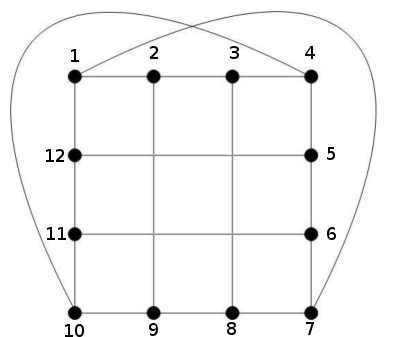
\includegraphics[width=0.3\textwidth]{include/graf.png}
			\caption*
{
\texttt{1: 2,7,12\\
2: 1,3,9\\
3: 2,4,8\\
4: 3,5,10\\
5: 4,6,12\\
6: 5,7,11\\
7: 1,6,8\\
8: 3,7,9\\
9: 2,8,10\\
10: 4,9,11\\
11: 6,10,12\\
12: 1,5,11}}
		\end{figure}
	\subsection{Wyjście programu}
	Wyjściem programu są:
	\begin{itemize}
	\item Odpowiedź na pytanie czy graf jest planarny.
	\item Jeżeli jest nieplanarny -  podgraf ściągalny do $K_5$ lub $K_{3,3}$ wyświetlany przy pomocą takiej samej reprezentacji jak graf wejściowy.
	\item Statystyki
		\begin{itemize}
		\item Czas obliczeń.
		\item Liczba operacji kluczowych (uznano za nią liczę wywołań funkcji rekurencyjnej \texttt{IsPlanar}).
		\end{itemize}
	\end{itemize}
	
\section{Zadany graf}

Zadany graf jest nieplanarny. Poniżej znajduje się reprezentacja podgrafu ściągalnego do $K_{3,3}$:

\begin{figure}[H]
\centering
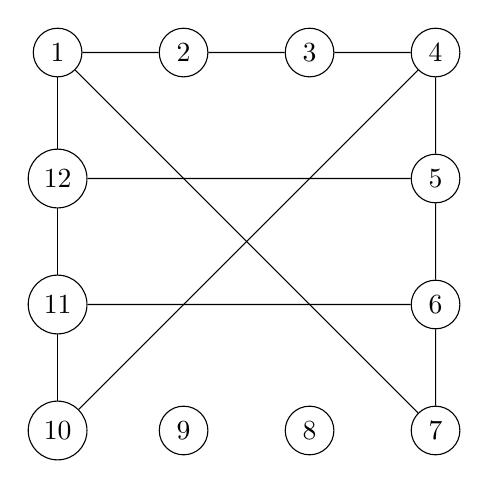
\begin{tikzpicture}
  [scale=.8,auto=left,every node/.style={draw,circle}]
  \node (n10) at (0,0) {10};
  \node (n9) at (2,0)  {9};
  \node (n8) at (4,0)  {8};
  \node (n7) at (6,0) {7};
  \node (n6) at (6,2)  {6};
  \node (n5) at (6,4)  {5};
  \node (n4) at (6,6) {4};
  \node (n3) at (4,6)  {3};
  \node (n2) at (2,6)  {2};
  \node (n1) at (0,6) {1};
  \node (n12) at (0,4)  {12};
  \node (n11) at (0,2)  {11};
  
  \foreach \from/\to in {n1/n2,n1/n7,n1/n12,n2/n3,n3/n4,n4/n5,n4/n10,n5/n6,n5/n12,n6/n7,n6/n11, n10/n11,n11/n12}
    \draw (\from) -- (\to);

\end{tikzpicture}

\caption*
{\textbf{Zadany graf}\\
\texttt
{1: 2,7,12\\
2: 1,3\\
3: 2,4\\
4: 3,5,10\\
5: 4,6,12\\
6: 5,7,11\\
7: 1,6\\
10: 4,11\\
11: 6,10,12\\
12: 1,5,11}}
\end{figure} 

Przedstawione zostaną ponadto kroki w jakich z wejściowego grafu poprzez operację ściągnięcia krawędzi 
otrzymano graf $K_{3,3}$. 
%\begin{description}
%\item[Graf wejściowy]\hfill

\begin{figure}[H]
\centering
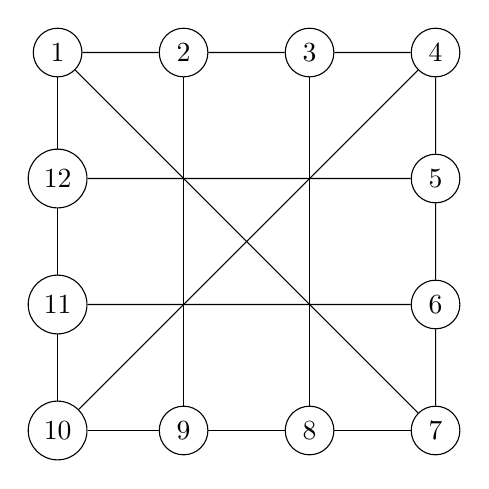
\begin{tikzpicture}
  [scale=.8,auto=left,every node/.style={draw,circle}]
  \node (n10) at (0,0) {10};
  \node (n9) at (2,0)  {9};
  \node (n8) at (4,0)  {8};
  \node (n7) at (6,0) {7};
  \node (n6) at (6,2)  {6};
  \node (n5) at (6,4)  {5};
  \node (n4) at (6,6) {4};
  \node (n3) at (4,6)  {3};
  \node (n2) at (2,6)  {2};
  \node (n1) at (0,6) {1};
  \node (n12) at (0,4)  {12};
  \node (n11) at (0,2)  {11};
  \foreach \from/\to in {n1/n2,n1/n7,n1/n12,n2/n3,n2/n9,n3/n4,n3/n8,n4/n5,n4/n10,n5/n6,n5/n12,n6/n7,n6/n11,n7/n8,n8/n9,n9/n10,n10/n11,n11/n12}
    \draw (\from) -- (\to);
\end{tikzpicture}
\caption*
{
\textbf{Graf wejściowy:}\\
\texttt
{1: 2,7,12\\
2: 1,3,9\\
3: 2,4,8\\
4: 3,5,10\\
5: 4,6,12\\
6: 5,7,11\\
7: 1,6,8\\
8: 3,7,9\\
9: 2,8,10\\
10: 4,9,11\\
11: 6,10,12\\
12: 1,5,11}}
\end{figure}


%\item[Ściągnięcie krawędzi (1,2)]\hfill

\begin{figure}[H]
\centering
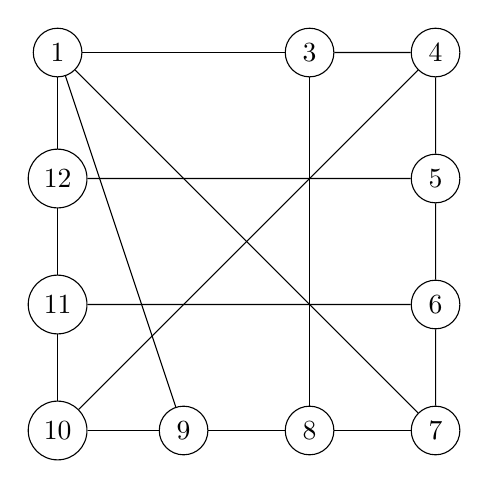
\begin{tikzpicture}
  [scale=.8,auto=left,every node/.style={draw,circle}]
  \node (n10) at (0,0) {10};
  \node (n9) at (2,0)  {9};
  \node (n8) at (4,0)  {8};
  \node (n7) at (6,0) {7};
  \node (n6) at (6,2)  {6};
  \node (n5) at (6,4)  {5};
  \node (n4) at (6,6) {4};
  \node (n3) at (4,6)  {3};
  \node (n1) at (0,6) {1};
  \node (n12) at (0,4)  {12};
  \node (n11) at (0,2)  {11};
  \foreach \from/\to in {n1/n3,n1/n7,n1/n9,n1/n12,n3/n4,n3/n8,n4/n5,n4/n10,n5/n6,n5/n12,n6/n7,n6/n11,n7/n8,n8/n9,n9/n10,n10/n11,n11/n12}
    \draw (\from) -- (\to);
\end{tikzpicture}
\caption*
{\textbf{Ściągnięcie krawędzi (1,2):}\\
\texttt
{1: 3,7,9,12\\
3: 1,4,8\\
4: 3,5,10\\
5: 4,6,12\\
6: 5,7,11\\
7: 1,6,8\\
8: 3,7,9\\
9: 1,8,10\\
10: 4,9,11\\
11: 6,10,12\\
12: 1,5,11}}
\end{figure} 

%\item[Ściągnięcie krawędzi (1,7)]\hfill

\begin{figure}[H]
\centering
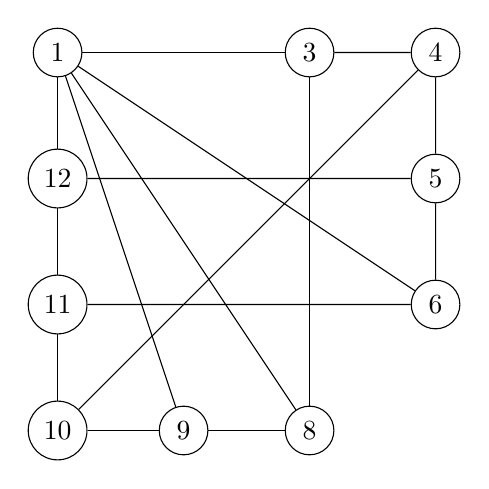
\begin{tikzpicture}
  [scale=.8,auto=left,every node/.style={draw,circle}]
  \node (n10) at (0,0) {10};
  \node (n9) at (2,0)  {9};
  \node (n8) at (4,0)  {8};
  \node (n6) at (6,2)  {6};
  \node (n5) at (6,4)  {5};
  \node (n4) at (6,6) {4};
  \node (n3) at (4,6)  {3};
  \node (n1) at (0,6) {1};
  \node (n12) at (0,4)  {12};
  \node (n11) at (0,2)  {11};
  \foreach \from/\to in {n1/n3,n1/n6,n1/n8,n1/n9,n1/n12,n3/n4,n3/n8,n4/n5,n4/n10,n5/n6,n5/n12,n6/n11,n8/n9,n9/n10,n10/n11,n11/n12}
    \draw (\from) -- (\to);
\end{tikzpicture}
\caption*
{\textbf{Ściągnięcie krawędzi (1,7):}\\
\texttt
{1: 3,6,8,9,12\\
3: 1,4,8\\
4: 3,5,10\\
5: 4,6,12\\
6: 1,5,11\\
8: 1,3,9\\
9: 1,8,10\\
10: 4,9,11\\
11: 6,10,12\\
12: 1,5,11}}
\end{figure} 

%\item[Ściągnięcie krawędzi (1,3)]\hfill

\begin{figure}[H]
\centering
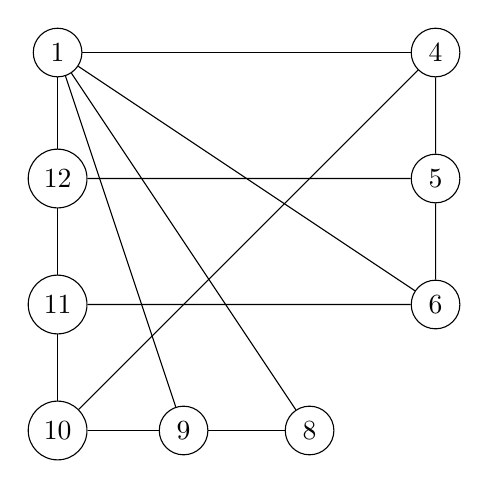
\begin{tikzpicture}
  [scale=.8,auto=left,every node/.style={draw,circle}]
  \node (n10) at (0,0) {10};
  \node (n9) at (2,0)  {9};
  \node (n8) at (4,0)  {8};
  \node (n6) at (6,2)  {6};
  \node (n5) at (6,4)  {5};
  \node (n4) at (6,6) {4};
  \node (n1) at (0,6) {1};
  \node (n12) at (0,4)  {12};
  \node (n11) at (0,2)  {11};
  \foreach \from/\to in {n1/n4,n1/n6,n1/n8,n1/n9,n1/n12,n4/n5,n4/n10,n5/n6,n5/n12,n6/n11,n8/n9,n9/n10,n10/n11,n11/n12}
    \draw (\from) -- (\to);
\end{tikzpicture}
\caption*
{\textbf{Ściągnięcie krawędzi (1,3):}\\
\texttt
{1: 4,6,8,9,12\\
4: 1,5,10\\
5: 4,6,12\\
6: 1,5,11\\
8: 1,9\\
9: 1,8,10\\
10: 4,9,11\\
11: 6,10,12\\
12: 1,5,11}}
\end{figure} 

%\item[Ściągnięcie krawędzi (1,9)]\hfill

\begin{figure}[H]
\centering
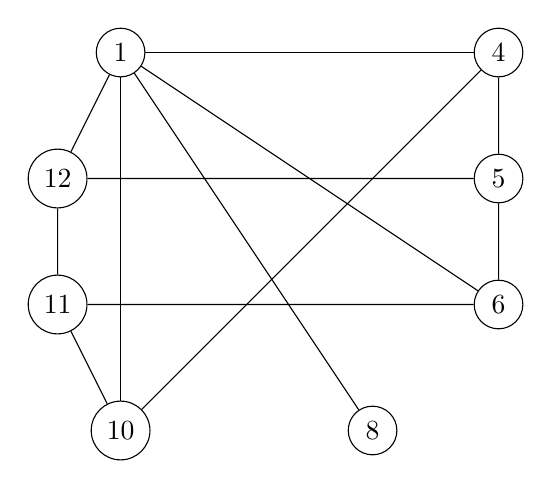
\begin{tikzpicture}
  [scale=.8,auto=left,every node/.style={draw,circle}]
  \node (n10) at (0,0) {10};
  \node (n8) at (4,0)  {8};
  \node (n6) at (6,2)  {6};
  \node (n5) at (6,4)  {5};
  \node (n4) at (6,6) {4};
  \node (n1) at (0,6) {1};
  \node (n12) at (-1,4)  {12};
  \node (n11) at (-1,2)  {11};
  \foreach \from/\to in {n1/n4,n1/n6,n1/n8,n1/n10,n1/n12,n4/n5,n4/n10,n5/n6,n5/n12,n6/n11,n10/n11,n11/n12}
    \draw (\from) -- (\to);
\end{tikzpicture}
\caption*
{\textbf{Ściągnięcie krawędzi (1,9):}\\
\texttt
{1: 4,6,8,10,12\\
4: 1,5,10\\
5: 4,6,12\\
6: 1,5,11\\
8: 1\\
10: 1,4,11\\
11: 6,10,12\\
12: 1,5,11}}
\end{figure} 

%\item[Ściągnięcie krawędzi (1,8)]\hfill

\begin{figure}[H]
\centering
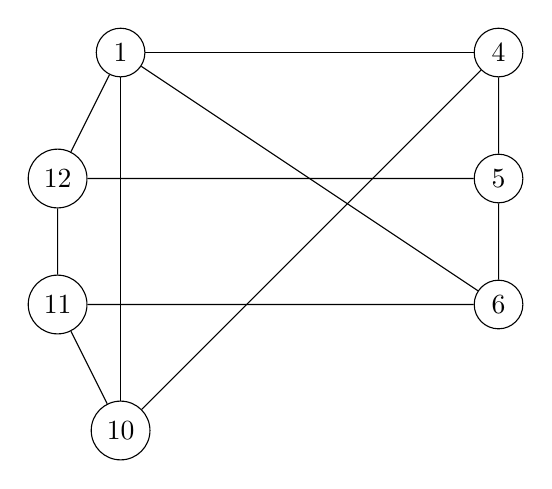
\begin{tikzpicture}
  [scale=.8,auto=left,every node/.style={draw,circle}]
  \node (n10) at (0,0) {10};
  \node (n6) at (6,2)  {6};
  \node (n5) at (6,4)  {5};
  \node (n4) at (6,6) {4};
  \node (n1) at (0,6) {1};
  \node (n12) at (-1,4)  {12};
  \node (n11) at (-1,2)  {11};
  \foreach \from/\to in {n1/n4,n1/n6,n1/n10,n1/n12,n4/n5,n4/n10,n5/n6,n5/n12,n6/n11,n10/n11,n11/n12}
    \draw (\from) -- (\to);
\end{tikzpicture}
\caption*
{\textbf{Ściągnięcie krawędzi (1,8):}\\
\texttt
{1: 4,6,10,12\\
4: 1,5,10\\
5: 4,6,12\\
6: 1,5,11\\
10: 1,4,11\\
11: 6,10,12\\
12: 1,5,11}}
\end{figure} 

%\item[Ściągnięcie krawędzi (4,10)]\hfill

\begin{figure}[H]
\centering
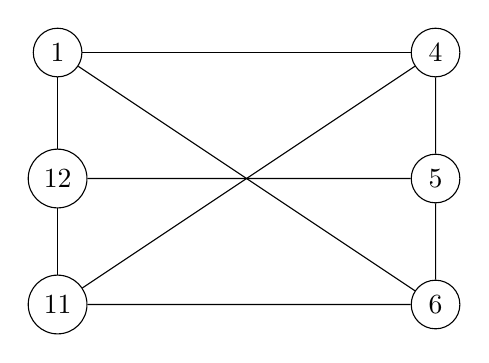
\begin{tikzpicture}
  [scale=.8,auto=left,every node/.style={draw,circle}]
  \node (n6) at (6,2)  {6};
  \node (n5) at (6,4)  {5};
  \node (n4) at (6,6) {4};
  \node (n1) at (0,6) {1};
  \node (n12) at (0,4)  {12};
  \node (n11) at (0,2)  {11};
  \foreach \from/\to in {n1/n4,n1/n6,n1/n12,n4/n5,n4/n11,n5/n6,n5/n12,n6/n11,n11/n12}
    \draw (\from) -- (\to);
\end{tikzpicture}
\caption*
{\textbf{Ściągnięcie krawędzi (4,10):}\\
\texttt
{1: 4,6,12\\
4: 1,5,11\\
5: 4,6,12\\
6: 1,5,11\\
11: 4,6,12\\
12: 1,5,11}}
\end{figure} 

%\end{description}

Po otrzymaniu grafu $K_{3,3}$ należało jeszcze znaleźć ściągalny do niego podgraf w grafie wejściowym. Robione to było podczas powrotów z funkcji rekurencyjnej. Oznaczmy otrzymany graf $K_{3,3}$ jako $H$, graf 
aktualnie będący argumentem funkcji rekurencyjnej jako $G$  i krawędź ściągniętą w danym kroku algorytmu z grafu $G$ jako $e = (e_1, e_2)$. 
W przypadku, gdy do grafu $H$ nie należy żaden z wierzchołków krawędzi $e$ graf $H$ nie jest zmieniany.
Gdy do grafu $H$ należy jeden z wierzchołków (dla ustalenia wagi przyjmijmy, że $e_1$) możliwe będzie rozszerzenie grafu $H$ o wierzchołek $e_2$. Dojdzie do tego wtedy i tylko wtedy, gdy w grafie $H$ istnieje pewne krawędź 
$(u,v)$, która nie istnieje w grafie $G$, ale za to w grafie $G$ istnieją krawędzie $(u,e_2)$ i ($v,e_2)$.  W takim przypadku w grafie $H$ przeprowadzone są następujące zmiany:
\begin{itemize}
\item Usuwana jest krawędź $(u,v)$.
\item Dodawany jest wierzchołek $e_2$.
\item Dodawane są wierzchołki $(u,e_2)$ i ($v,e_2)$.
\end{itemize} 

Zgodnie z powyższym opisem dla zadanego grafu odtworzenie podgrafu ściągalnego do $K_{3,3}$ przebiegało w następujących krokach. 
\begin{description}
\item[Graf $K_{3,3}$] \hfill \\
\begin{verbatim}
1: 4,6,12
4: 1,5,11
5: 4,6,12
6: 1,5,11
11: 4,6,12
12: 1,5,11
\end{verbatim}
\item[Ściągnięcie krawędzi (4,10)] \hfill \\
\begin{verbatim}
1: 4,6,12
4: 1,5,10
5: 4,6,12
6: 1,5,11
10: 4,11
11: 6,10,12
12: 1,5,11	
\end{verbatim}
\item[Ściągnięcie krawędzi (1,8)] \hfill \\
\begin{verbatim}
1: 4,6,12
4: 1,5,10
5: 4,6,12
6: 1,5,11
10: 4,11
11: 6,10,12
12: 1,5,11	
\end{verbatim}
\item[Ściągnięcie krawędzi (1,9)] \hfill \\
\begin{verbatim}
1: 4,6,12
4: 1,5,10
5: 4,6,12
6: 1,5,11
10: 4,11
11: 6,10,12
12: 1,5,11	
\end{verbatim}
\item[Ściągnięcie krawędzi (1,3)] \hfill \\
\begin{verbatim}
1: 3,6,12
3: 1,4
4: 3,5,10
5: 4,6,12
6: 1,5,11
10: 4,11
11: 6,12,10
12: 1,5,11
\end{verbatim}
\item[Ściągnięcie krawędzi (1,7)] \hfill \\
\begin{verbatim}
1: 3,7,12
3: 1,4
4: 3,5,10
5: 4,6,12
6: 5,7,11
7: 1,6
10: 4,11
11: 6,12,10
12: 1,5,11
\end{verbatim}
\item[Ściągnięcie krawędzi (1,2)] \hfill \\
\begin{verbatim}
1: 2,7,12
2: 1,3
3: 2,4
4: 3,5,10
5: 4,6,12
6: 5,7,11
7: 1,6
10: 4,11
11: 6,12,10
12: 1,5,11
\end{verbatim}
\end{description}

\section{Bibliografia}

	[1]	Wilson R. J., Wprowadzenie do teorii grafów, Warszawa 1998, Wydawnictwo Naukowe PWN.\\[0.3cm]
	[2]	\url{http://www.akira.ruc.dk/~keld/teaching/algoritmedesign\_f08/Artikler/06/Hopcroft73.pdf}, ost. wiz. 27.01.2013\\[0.3cm] 
	[3]	\url{http://jgaa.info/accepted/2004/BoyerMyrvold2004.8.3.pdf}, ost. wiz. 27.01.2013 \\[0.3cm]
	[4]	\url{www.win.tue.nl/~nikhil/courses/2012/2WO08/lecture5.pdf}, ost. wiz. 17.12.2013.\\[0.3cm]

\end{document}	
